\documentclass[psamsfonts]{amsart}

%-------Packages---------
\usepackage{amssymb,amsfonts}
\usepackage[all,arc]{xy}
\usepackage{enumerate}
\usepackage{mathrsfs}
\usepackage[utf8]{inputenc}
\usepackage{amsfonts}
\usepackage{amsmath}
\usepackage[shortlabels]{enumitem}
\usepackage{graphicx}
\usepackage{xcolor}
\usepackage{mdframed}
\usepackage{float}
\usepackage[margin=0.75in]{geometry}
\usepackage{subfigure}

%%% hyperref stuff is taken from AGT style file
\usepackage{hyperref}  
\hypersetup{%
  bookmarksnumbered=true,%
  bookmarks=true,%
  colorlinks=true,%
  linkcolor=blue,%
  citecolor=blue,%
  filecolor=blue,%
  menucolor=blue,%
  pagecolor=blue,%
  urlcolor=blue,%
  pdfnewwindow=true,%
  pdfstartview=FitBH}   
  
\let\fullref\autoref
%
%  \autoref is very crude.  It uses counters to distinguish environments
%  so that if say {lemma} uses the {theorem} counter, then autrorefs
%  which should come out Lemma X.Y in fact come out Theorem X.Y.  To
%  correct this give each its own counter eg:
%                 \newtheorem{theorem}{Theorem}[section]
%                 \newtheorem{lemma}{Lemma}[section]
%  and then equate the counters by commands like:
%                 \makeatletter
%                   \let\c@lemma\c@theorem
%                  \makeatother
%
%  To work correctly the environment name must have a corrresponding 
%  \XXXautorefname defined.  The following command does the job:
%
\def\makeautorefname#1#2{\expandafter\def\csname#1autorefname\endcsname{#2}}
%
%  Some standard autorefnames.  If the environment name for an autoref 
%  you need is not listed below, add a similar line to your TeX file:
%  
%\makeautorefname{equation}{Equation}%
\def\equationautorefname~#1\null{(#1)\null}
\makeautorefname{footnote}{footnote}%
\makeautorefname{item}{item}%
\makeautorefname{figure}{Figure}%
\makeautorefname{table}{Table}%
\makeautorefname{part}{Part}%
\makeautorefname{appendix}{Appendix}%
\makeautorefname{chapter}{Chapter}%
\makeautorefname{section}{Section}%
\makeautorefname{subsection}{Section}%
\makeautorefname{subsubsection}{Section}%
\makeautorefname{theorem}{Theorem}%
\makeautorefname{thm}{Theorem}%
\makeautorefname{sta}{Statement}%
\makeautorefname{cor}{Corollary}%
\makeautorefname{lem}{Lemma}%
\makeautorefname{prop}{Proposition}%
\makeautorefname{pro}{Property}
\makeautorefname{conj}{Conjecture}%
\makeautorefname{conj}{Convention}%
\makeautorefname{defn}{Definition}%
\makeautorefname{notn}{Notation}
\makeautorefname{notns}{Notations}
\makeautorefname{rem}{Remark}%
\makeautorefname{rems}{Remarks}%
\makeautorefname{quest}{Question}%
\makeautorefname{exmp}{Example}%
\makeautorefname{ax}{Axiom}%
\makeautorefname{claim}{Claim}%
\makeautorefname{ass}{Assumption}%
\makeautorefname{asses}{Assumptions}%
\makeautorefname{con}{Construction}%
\makeautorefname{prob}{Problem}%
\makeautorefname{warn}{Warning}%
\makeautorefname{obs}{Observation}%
\definecolor{problem}{rgb}{0.8,0.8,0.8}
\newcommand{\comp}[2]{
\vspace{0.2in}\begin{mdframed}[
  backgroundcolor=problem,
  userdefinedwidth=10cm,
  align=center,
  skipabove=\topsep,
  skipbelow=\topsep
  ]
  \emph{{#1}:\newline} {#2}
\end{mdframed}}

%
%                  *** End of hyperref stuff ***

%theoremstyle{plain} --- default
\newtheorem{thm}{Theorem}[section]
\newtheorem{sta}{Statement}[section]
\newtheorem{cor}{Corollary}[section]
\newtheorem{prop}{Proposition}[section]
\newtheorem{lem}{Lemma}[section]
\newtheorem{prob}{Problem}[section]
\newtheorem{conj}{Conjecture}[section]

\theoremstyle{definition}
\newtheorem{defn}{Definition}[section]
\newtheorem{conv}{Convention}[section]
\newtheorem{ass}{Assumption}[section]
\newtheorem{asses}{Assumptions}[section]
\newtheorem{ax}{Axiom}[section]
\newtheorem{con}{Construction}[section]
\newtheorem{exmp}{Example}[section]
\newtheorem{notn}{Notation}[section]
\newtheorem{notns}{Notations}[section]
\newtheorem{pro}{Property}[section]
\newtheorem{quest}{Question}[section]
\newtheorem{rem}{Remark}[section]
\newtheorem{rems}{Remarks}[section]
\newtheorem{warn}{Warning}[section]
\newtheorem{sch}{Scholium}[section]
\newtheorem{obs}{Observation}[section]

%%%% hack to get fullref working correctly
\makeatletter
\let\c@obs=\c@thm
\let\c@cor=\c@thm
\let\c@prop=\c@thm
\let\c@lem=\c@thm
\let\c@prob=\c@thm
\let\c@con=\c@thm
\let\c@conj=\c@thm
\let\c@defn=\c@thm
\let\c@notn=\c@thm
\let\c@notns=\c@thm
\let\c@exmp=\c@thm
\let\c@ax=\c@thm
\let\c@pro=\c@thm
\let\c@ass=\c@thm
\let\c@warn=\c@thm
\let\c@rem=\c@thm
\let\c@conv=\c@thm
\let\c@sch=\c@thm
\numberwithin{equation}{section}
\makeatother



\bibliographystyle{plain}

%--------Meta Data: Fill in your info------
\title{Optimal Transport and Wasserstein Space}

\author{Aidan Copinga}

\date{2/5/2022 DEADLINES: Draft MARCH 28, 2022 and Final version MAY 6, 2022}

\begin{document}

\begin{abstract}

In the 18th century, a problem was created about the best way to transport munitions to each barracks in France. This problem, now called optimal transportation, has shown useful in many fields of mathematics, from PDEs to image processing and machine learning.
In the most simple terms, the optimal transport problem is just that-what is the optimal way to transport items from one place to another. Typically, we call these transport maps. That being said, it has quite rigorous and fascinating mathematical consequences.

\end{abstract}

\maketitle

\tableofcontents

\section{Formulation of Optimal Transport}
\subsection{Problem}\hfill\\

Start with a simple example where we have a pile of dirt, and a hole to fill completely with the dirt.
To transport the dirt from this pile to the hole, clearly, the volume of the hole and the pile must be the same. As is suggested in \autoref{villani}, we normalize this mass to $1$.\newline
To model this rigorously, allow the pile to be space $X$ and the hole to be space $Y$. It's natural to define probability measures $\mu,\nu$ on $X,Y$ respectively.
In other words, for measurable $A\subset X$ and $B\subset Y$, $\mu(A)$ is the volume in the pile $X$ and $\nu(B)$ is the volume to be filled in hole $Y$.\newline
Now, introduce cost function $c: X\times Y \to \mathbb{R}$ such that for points $x\in X,y\in Y$, $c(x,y)$ represents how much energy is exhausted transporting point $x$ in the pile to point $y$ in the hole.\newline
We can now introduce the transportation problem.
%\comp{}{Given $n$ piles of sand and $m$ holes to be filled completely.}
\begin{defn}[Transportation Problem]\label{defn:tp}
Given measure spaces $X,Y$ and $\mu,\nu$ respectively on $X,Y$ and $c: X\times Y\to \mathbb{R}$. The Transportation Problem is realizing the transport plan from Figure \ref{fig:tran} while minimizing $c$.
\end{defn}
\begin{figure}[H]
  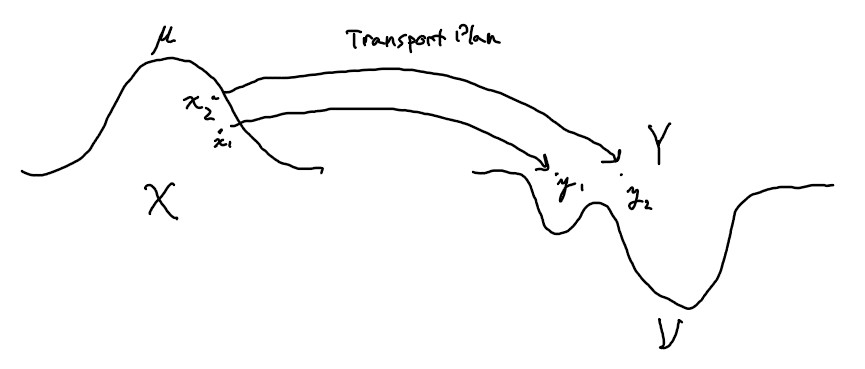
\includegraphics[scale=0.3]{transport.jpg}
  \caption{Transportation Problem}
  \label{fig:tran}
\end{figure}

There are two primary formulation for the transportation problem, the Monge and the Kantorovich formulation. The Monge formulation came historically before Kantorovich's, so I will be introducing it first.
\subsection{Monge Formulation}\hfill\\

\autoref{fig:tran} uses the Lagrangian framework in order to describe \autoref{defn:tp}. What this means is that particles $x\in X$ are observed individually as they are transported to $y\in Y$, and importantly, mass cannot be split, or the flows $T: X\to Y$ must be bijective.\newline From here, we introduce
the Monge formulation, which observes a transport map $T$ that transports $\mu$ to $\nu$. Before we define it, we must define what is meant by transporting one measure to another.
\begin{defn}[Transport Maps]\label{defn:transport_map}
  We say that $T: X\to Y$ transports $\mu\in \mathcal{P}(X)$ to $\nu\in\mathcal{P}(Y)$ if 
  \begin{equation*}\label{eqn:pushforward}
    \mu(T^{-1}(B)) = \nu(B) \quad\text{for all $\nu$-measurable $B\in Y$.}
  \end{equation*}
  This is typically called the \textit{pushforward} of $\mu$ and denoted as $T_\#\mu$.
\end{defn} 
In order to describe the Monge Formulation, we denote the set of all $T$ such that $T_\#\mu=\nu$ with
\begin{equation}
  \mathcal{T}(\mu,\nu) = \left\{T: X\to Y \vert T_\#\mu = \nu,\,\,\text{$T$ measurable} \right\}
\end{equation}
\begin{defn}[Monge Formulation of the transport problem]\label{defn:monge}
  \begin{equation}
    \underset{\mathcal{T}(\mu,\nu)}{\text{minimize}}\left\{\int_X c(x,T(x))d\mu(x)\right\}
  \end{equation}
\end{defn}
In other words, \autoref{defn:monge} is minimizing the energy required from transporting $X\overset{T(x)}{\to}Y$. 
\begin{exmp}[Dirt piles in the Monge case]
  Let's consider that on a high level, transport maps are the method one uses to move dirt from $X$ to a hole in $Y$ and $c$ can be the time required.\newline
  We see that if the transport map were moving every individual dirt particle into a hole in $Y$, the amount of time required would be substantial compared to 
  a method such as using a shovel to transport many dirt particles to a hole in $Y$.\newline 
  Importantly, however, in every transport map, dirt particles (or a set of particles) are transported to exactly one hole. This is what's happening in \autoref{fig:tran}.
\end{exmp}
\subsection{Kantorovich Formulation}\hfill\\

It's natural to ask what happens on the product space $X\times Y$. The Kantorovich does exactly this by defining \textit{transportation plans} as a product measure on $X\times Y$.

\begin{defn}[Transport Plans]
  A transport plan, $\pi \in \mathcal{P}(X\times Y)$, is valid if all mass taken from a point $x\in X$ must correspond to $d\mu(x)$ and all mass taken from a point $y\in Y$ must correspond to $d\nu(y)$, or in other terms,
  \begin{equation}\label{eqn:const}
    \pi(A\times Y) = \mu(A)\quad \pi(X\times B) = \nu(B).
  \end{equation}
\end{defn}
  
To define  Kantorovich's Formulation, we define the set of all probability measures that follow \autoref{eqn:const} with
\begin{equation}
  \Pi(\mu,\nu) = \left\{\pi\in \mathcal{P}(X\times Y): \text{\autoref{eqn:const} holds for all measurable $A\subset X$, $B\subset Y$}\right\}.
\end{equation}
\begin{defn}[Kantorovich Formulation of the transport problem]\label{defn:kantorovich}
  \begin{equation}
    \underset{\Pi(\mu,\nu)}{\text{minimize}}\left\{\int_{X\times Y} c(x,y)d\pi(x,y)\right\}.
  \end{equation}
\end{defn}
This formulation is typically referred to as a relaxation of \autoref{defn:monge}, or that Monge's problem is stronger than Kantorovich's.
\begin{prop}\label{prop:equiv}
  The Monge Formulation can be written as a Kantorovich Formulation.
\end{prop}
\begin{proof}
  Because mass cannot be split in the Monge Formulation, this means that we can rewrite $d\pi(x,y)$ in Definition \ref{defn:kantorovich}
  with
  \[ d\pi(x,y)=d\pi_T(x,y) \equiv d\mu(x)\delta[y=T(x)]\]
  where $\delta$ is the dirac measure and $T(x)$ is as defined in \autoref{defn:transport_map}. As $\int_Y\xi(x,y)\delta[y=T(x)] = \xi(x,T(x))$ for any nonnegative function $\xi:X\times Y\to \mathbb{R}$, we have that 
  \[ \int_{X\times Y}c(x,y)d\pi(x,y) = \int_X c(x,T(x))d\mu(x).\]
  In order for $\pi_T$ to be in $\Pi(\mu,\nu)$, we consider \autoref{eqn:const}
  \[\pi(A\times Y) = \mu(A)\quad \pi(X \times B) = \nu(B)\]
  so we see that this is the case where we have measurable $B\in Y$ with 
  \[\nu(B) = \mu(T^{-1}(B)).\]
  Of course, we allowed $T(x)$ to follow \autoref{defn:transport_map}, so this condition is satisfied. Furthermore, this is equivalent to the Kantorovich formulation of the transportation problem.
\end{proof}
We see that the Monge Formulation is the stronger case, where we restrict mass in $X$ from being able to be split. However, \autoref{prop:equiv} can also be framed as stating that a Kantorovich Formulation with mass
that cannot be split is a Monge Problem.
\begin{exmp}[Dirt Piles in the Kantorovich Case]
  Because now we're dealing with product measures, it's natural to think about the case where mass is split. One way to think about this the transport plan of using a larger
  shovel that may hold too much mass for one hole, but can hold enough to fill multiple. This is equivalent to the mass in the shovel being some product measure in $\Pi$, where 
  now transport is dependent on both $X$ and $Y$. This is described in \autoref{fig:kant}.
  \begin{figure}[H]
    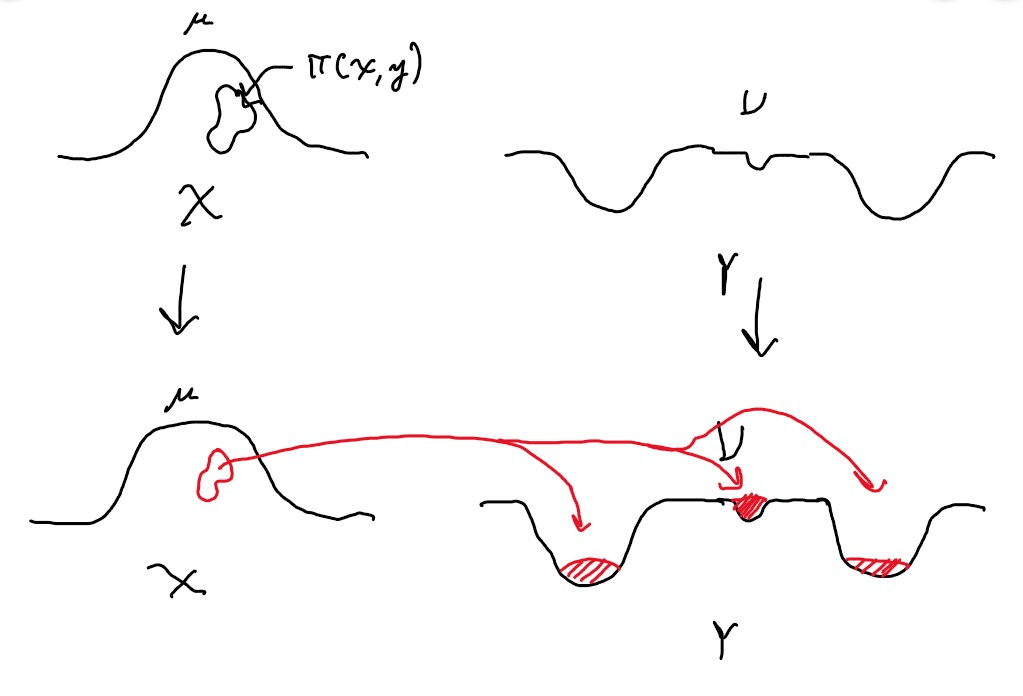
\includegraphics[scale=0.3]{kantorovich.jpg}
    \caption{We see in this case the mass $\pi(x,y)$ has been split into multiple holes in $Y$ between steps where red denotes the mass added to $Y$ and subtracted from $X$.}
    \label{fig:kant}
  \end{figure}
\end{exmp} 
\section{Kantorovich Duality}

For linear optimization problems, it is well known that they admit a dual problem, and Kantorovich in 1942 showed duality for \autoref{defn:kantorovich} for $c(x,y) = d(x,y)$ where $d$ is the distance metric, but it still holds in generality. 
To begin to understand Kantorovich's dual problem, we can think of Caffarelli's Shipper's Problem described in \autoref{bib:villani}
\begin{exmp}[Shipper's Problem]\label{exmp:ship}
  It costs $c(x_1,y_1)$ dollars for a factory to transport coal from mine $x_1$ to factory $y_1$. I tell the mine owner that I can charge them $\phi(x_1)$ dollars to pick up at mine $x_1$ and charge $\psi(y_1)$ to deliver to factory $y_1$, then, in order for the factory owner to agree to my terms, 
  \[\phi(x)+\psi(y)\le c(x,y)\]
  for every location $x$ and destination $y$. However, I can make this sum as close as I want to $c(x,y)$ because I have the liberty to choose $\phi,\psi$. In other words, the most money I can make is equal to the least effort it would take the factory owner (just simply transporting it with cost $c(x,y)$) which is exactly what a dual problem would suggest.
\end{exmp}
\subsection{Kantorovich Duality}
\begin{thm}[Kantorovich Duality]\label{thm:kant}
Let $X$ and $Y$ be Polish spaces, let $\mu\in \mathcal{P}(X)$ and $\nu\in\mathcal{P}(Y)$, and let\hfill\break $c: X\otimes Y\to \mathbb{R}^+\cup\{+\infty\}$ be a lower semicontinuous cost function.

  Whenever $\pi \in \mathcal{P}(X\otimes Y)$ and $(\phi,\psi)\in L^1(d\mu)\otimes L^1(d\nu)$, define 
  \[I(\pi)= \int_{X\otimes Y}c(x,y)d\pi(x,y),\quad J(\phi,\psi) = \int_X\phi d\mu + \int_Y\psi d\nu.\]
  Define $\Pi(\mu,\nu)$ to be the set of all Borel probability measures $\pi$ on $X\otimes Y$ such that for all measurable subsets $A\subset X$ and $B\subset Y$,
  \[\pi(A\otimes Y) = \mu(A),\quad \pi(X\otimes B)= \nu(B),\]
  and define $\Phi_c$ to be the set of all measurable functions $(\phi,\psi)$ satisfying
  \begin{equation}
    \phi(x) + \psi(y) \le c(x,y)
  \end{equation}
  for $d\mu-$almost every $x\in X$, $d\nu-$almost every $y\in Y$. Then,
  \begin{equation}
    \inf_{\Pi(\mu,\nu)} I(\pi) = \sup_{\Phi_c}{J(\phi,\psi)}.
  \end{equation}
\end{thm}
It is not a priori clear that $\sup J$ is the same upon restricting $\Phi_c$ to bounded continuous functions $C_b$, so we'll consider $\Phi_c\cap C_b$ and $\Phi_c\cap L^1$. With this,
we can begin the proof.
\begin{prop}[Easy part of Kantorovich Duality]\label{prop:kant}
  Under the same assumptions as \autoref{thm:kant},
  \begin{equation}
    \sup_{\Phi_c \cap C_b} J(\phi,\psi) \le \sup_{\Phi_c\cap L^1} J(\phi,\psi) \le \inf_{\Pi(\mu,\nu)}I[\pi].
  \end{equation}
\end{prop}
\begin{proof}
  $C_b(X)\times C_b(Y) \subset L^1(X)\times L^1(Y)$ so the left inequality is trivial. 
\end{proof}
\section{Existence of Transport Plans/Maps}
\subsection{Existence of Transport Plans}
\subsection{Brenier / Knott-Smith Optimality}
\section{Wasserstein}
\subsection{Wasserstein Distances}
\subsection{Wasserstein Topology}
\section{Gradient Flows and PDEs}
\subsection{Gradient Flow Motivation}
\subsection{Benamou-Brenier Theorem}
\section{Writing}  Before getting to latex comments, I'll say a few words about writing, venting from many years of hard experience. 

It is important that what you write is something you would actually like to read.  There should be no overuse of symbols.
Clusters of symbols can be barbaric.  There are subjects whose literature is festooned with sentences written almost entirely with symbols like $\exists$, $\forall$.  Don't do that. Never use a symbol for a verb.  Never start a sentence with a symbol or with the word ``And''.

Grammar should be correct.  Never start a sentence with ``Where ...".   
Mismatches of singular and plural are excruciatingly painful, utterly abhorrent.  You cannot write
``Let ..., then ..."  That is what is called a run-on sentence. You must write ``Let ... .  Then ... ."
Alternatively, ``If ..., then ..."  works just fine.

Avoid words or phrases like Simply, Obviously, Just, ..., It is easy to see.  They serve only to intimidate or to browbeat the reader into acquiescence. 
Especially if English is not your native language, make sure you have  somebody fluent in English check what you have written.     

References to numbered statements are best in the form Theorem 2.3, not just 2.3.  Use  \verb|usepackage{hyperref}| to get this right.  Really.  I will likely return papers unread that don't. 
Equations should be referred to as (2.3), NOT 2.3 or equation 2.3 or equation (2.3).


Bad writing makes for unpleasant papers, no matter how good the material.

\section*{Acknowledgments}  You should thank anyone who deserves thanks, and for sure you should
thank your mentor.   ``It is a pleasure to thank my mentor, 
his/her name, for ....  ".   Or add anyone else, for example ``I thank [another participant] for helping 
me understand [something or other]"

\section{bibliography}  The bibliography should list all sources that you have used and referenced.
And you should reference anything you use.   Especially if you quote any result without proof, you MUST
give a reference.   And never ever should you copy material directly or more or less directly, from a source.

\begin{thebibliography}{9}

\bibitem{ams} http://www.ams.org/publications/authors/tex/amslatex

\bibitem{amsshort}
Michael Downes.
Short Math Guide for \LaTeX.
http://tex.loria.fr/general/downes-short-math-guide.pdf

\bibitem{May}
J. P. May.
A Concise Course in Algebraic Topology.
University of Chicago Press. 1999. 

\bibitem{notsoshort}
Tobias Oekiter, Hubert Partl, Irene Hyna and Elisabeth Schlegl.
The Not So Short Introduction to \LaTeX 2e.
https://tobi.oetiker.ch/lshort/lshort.pdf

\end{thebibliography}

\end{document}

